\documentclass{article}
\usepackage{graphicx}
\usepackage{caption}
\usepackage{xcolor}
\usepackage{hyperref}

\hypersetup{
    colorlinks=true,
    urlcolor={blue!90!black},
}

\title{ZK University \\[4pt] \normalsize\textsc{Initial Submission}}
\author{André Dal Bosco}

\begin{document}
\maketitle

\section*{A. Conceptual Knowledge}

\subsection*{What is a smart contract?}

Let's talk about what a contract is. A contract can be seen as an agreement between two or more parties which describes possibly various situations, and dictates what is to be done about them. Let me show two examples:
\begin{itemize}
    \item Contract between Alice and Bob

    Every time Alice gives Bob an apple, Bob will give Alice an orange, except when Bob has no oranges left.
    
    \item Contract describing a poker game
    
    Players initially stake some money to play the poker game. The winner takes all the money.
\end{itemize}
        
Now there's two problems with these contracts: there must be some way to enforce it; thus, if Bob doesn't give back Alice an orange, the government could, for example, could threat arresting Bob, in an effort to enforce such a contract. Another point is that people may have different interpretations of the contract, so Bob may think, for example, that it's okay to give Alice a lemon instead of an orange, if he considers the oranges and lemons to be equivalent. Two key properties of smart contracts are that they are enforced without use of third parties, and that they are unambiguous. Once a smart contract is 'signed', it's not up to some party to enforce the contract, but to the contract itself, and although this sounds kinda weird, it's the way it works.

You could think of this like a seed. If you plant an apple seed, you'll have an apple tree, although you may have wanted a peach tree. It's not up to anyone to enforce that seed to become an apple tree, but it is somehow already encoded into the seed that it will become an apple tree. Because of this special property, we call this contract a \emph{smart contract}.

A smart contract is deployed by first being rewritten in a way that computers can read better, called bytecode, then doing an operation called transaction containing this bytecode in which there is no recipient. A transaction is basically an operation where data is comitted to a special network called blockchain. Once in the chain, anyone is able to interact with this smart contract.

\subsection*{What is gas?}

Suppose you wanna go on a trip by car with your family all around your country. It's obvious that gas will be necessary for the trip, since it's what moves the car. Moreover, during the trip, you might have to refuel the car, and the price might be different in different cities. Of course, the gas will make the car move, because it has some hidden energy, that is somehow liberated by the engine of the car.

An Ethereum transaction functions in a similar way. The contract could for example, specify the cities through which the car will pass, and people called miners would represent the car. The miners might choose people that provide more gas, because they'll have more chance of actually having enough gas to make the trip. Someone with not enough gas will not be chosen to make the trip. Additionally, the miners might be interested in some kind of tip for their service, and this can be included with the gas.

There is a crucial difference though. Gas in Ethereum does not carry some kind of hidden power, so it's possible some part of this gas actually goes to the miner, as a type of payment.

If you make just one trip per year, than it's okay if you use a little bit more gas than necessary. But what about your dad, that goes to work everyday? Over the course of time, small savings can add up, so he will probably prefer a car that spends less gas. A smart contract is generally something that can possibly be executed a considerable amount of times, so that it's in our best interest to optmize it. If we improve gas consumption of a smart contract by overall 1\%, it might not make much difference for a single transaction, but suppose that the contract is execute 10000 a day. Then basically we would be saving gas equivalent to 100 executions of this contract, which is considerable. 

\subsection*{What is a hash?}

Imagine you have some different color paint, and you mix them in some way to that you produce a new color. If you give someone else the exact colors and proportions you used, they'll be able to produce the same final color very efficiently, and anyone who sees this new produced color won't be able to guess exactly what colors you used in the mix.

A hash is basically a function which gets some input and returns some output. Given the same input, it'll produce the same output. The same is valid for our mixture process, so it could be seen as some type of hashing function.

Hashing is generally used when you have a lot of information that you have to put in different buckets efficiently. Suppose you analyse subgroups of 2 colors in a group of 10 colors. You might try to organize them into buckets, but how to do that? Well, you could mix these two colors and try to use some property of the final color to do this organization. For example, if you have 2 buckets, you could say that if the color is lighter than some threshold, than it will be put in the first bucket, otherwise in the second bucket.

\subsection*{How would you prove to a colorblind person that two different colored objects are actually of different colors?}

Suppose I have two objects, A and B, of different colors that I can distinguish because they are of different colors, but which I know the colorblind person won't be able to distinguish. Of course, it's not enough to just assert to this person that the colors are different, because he won't necessarily trust me. I'll need to do something that proves that I actually know of this privileged information of which he does not possess, which is actually seeing that the two objects are of different colors.

If I let him have A and B, he can examine the objects so he verifies they are apparently identic, and let him choose one of the objects. Suppose he chooses A. To test whether I really know how to differentiate these objects, he may hide both, randomly switch them, and then present them to me. He can keep track which object is A and which is B, but if the objects are equal, I shouldn't be able to tell him which is which, but I can, since they are of different colors. Initially, if I get my guess right, he may think it might be just luck, but with enough iterations of this process, he will eventually be convinced something more than chance is at play, that is, my assertion that objects are of different colors must be right.

\newpage

\section*{B. Solidity}

The first part of the Solidity assignment is a set/get contract. The code can be found \href{https://github.com/dbsc/zku/blob/main/background_assignment/helloworld.sol}{here}.

\begin{figure}[h]
    \centering
    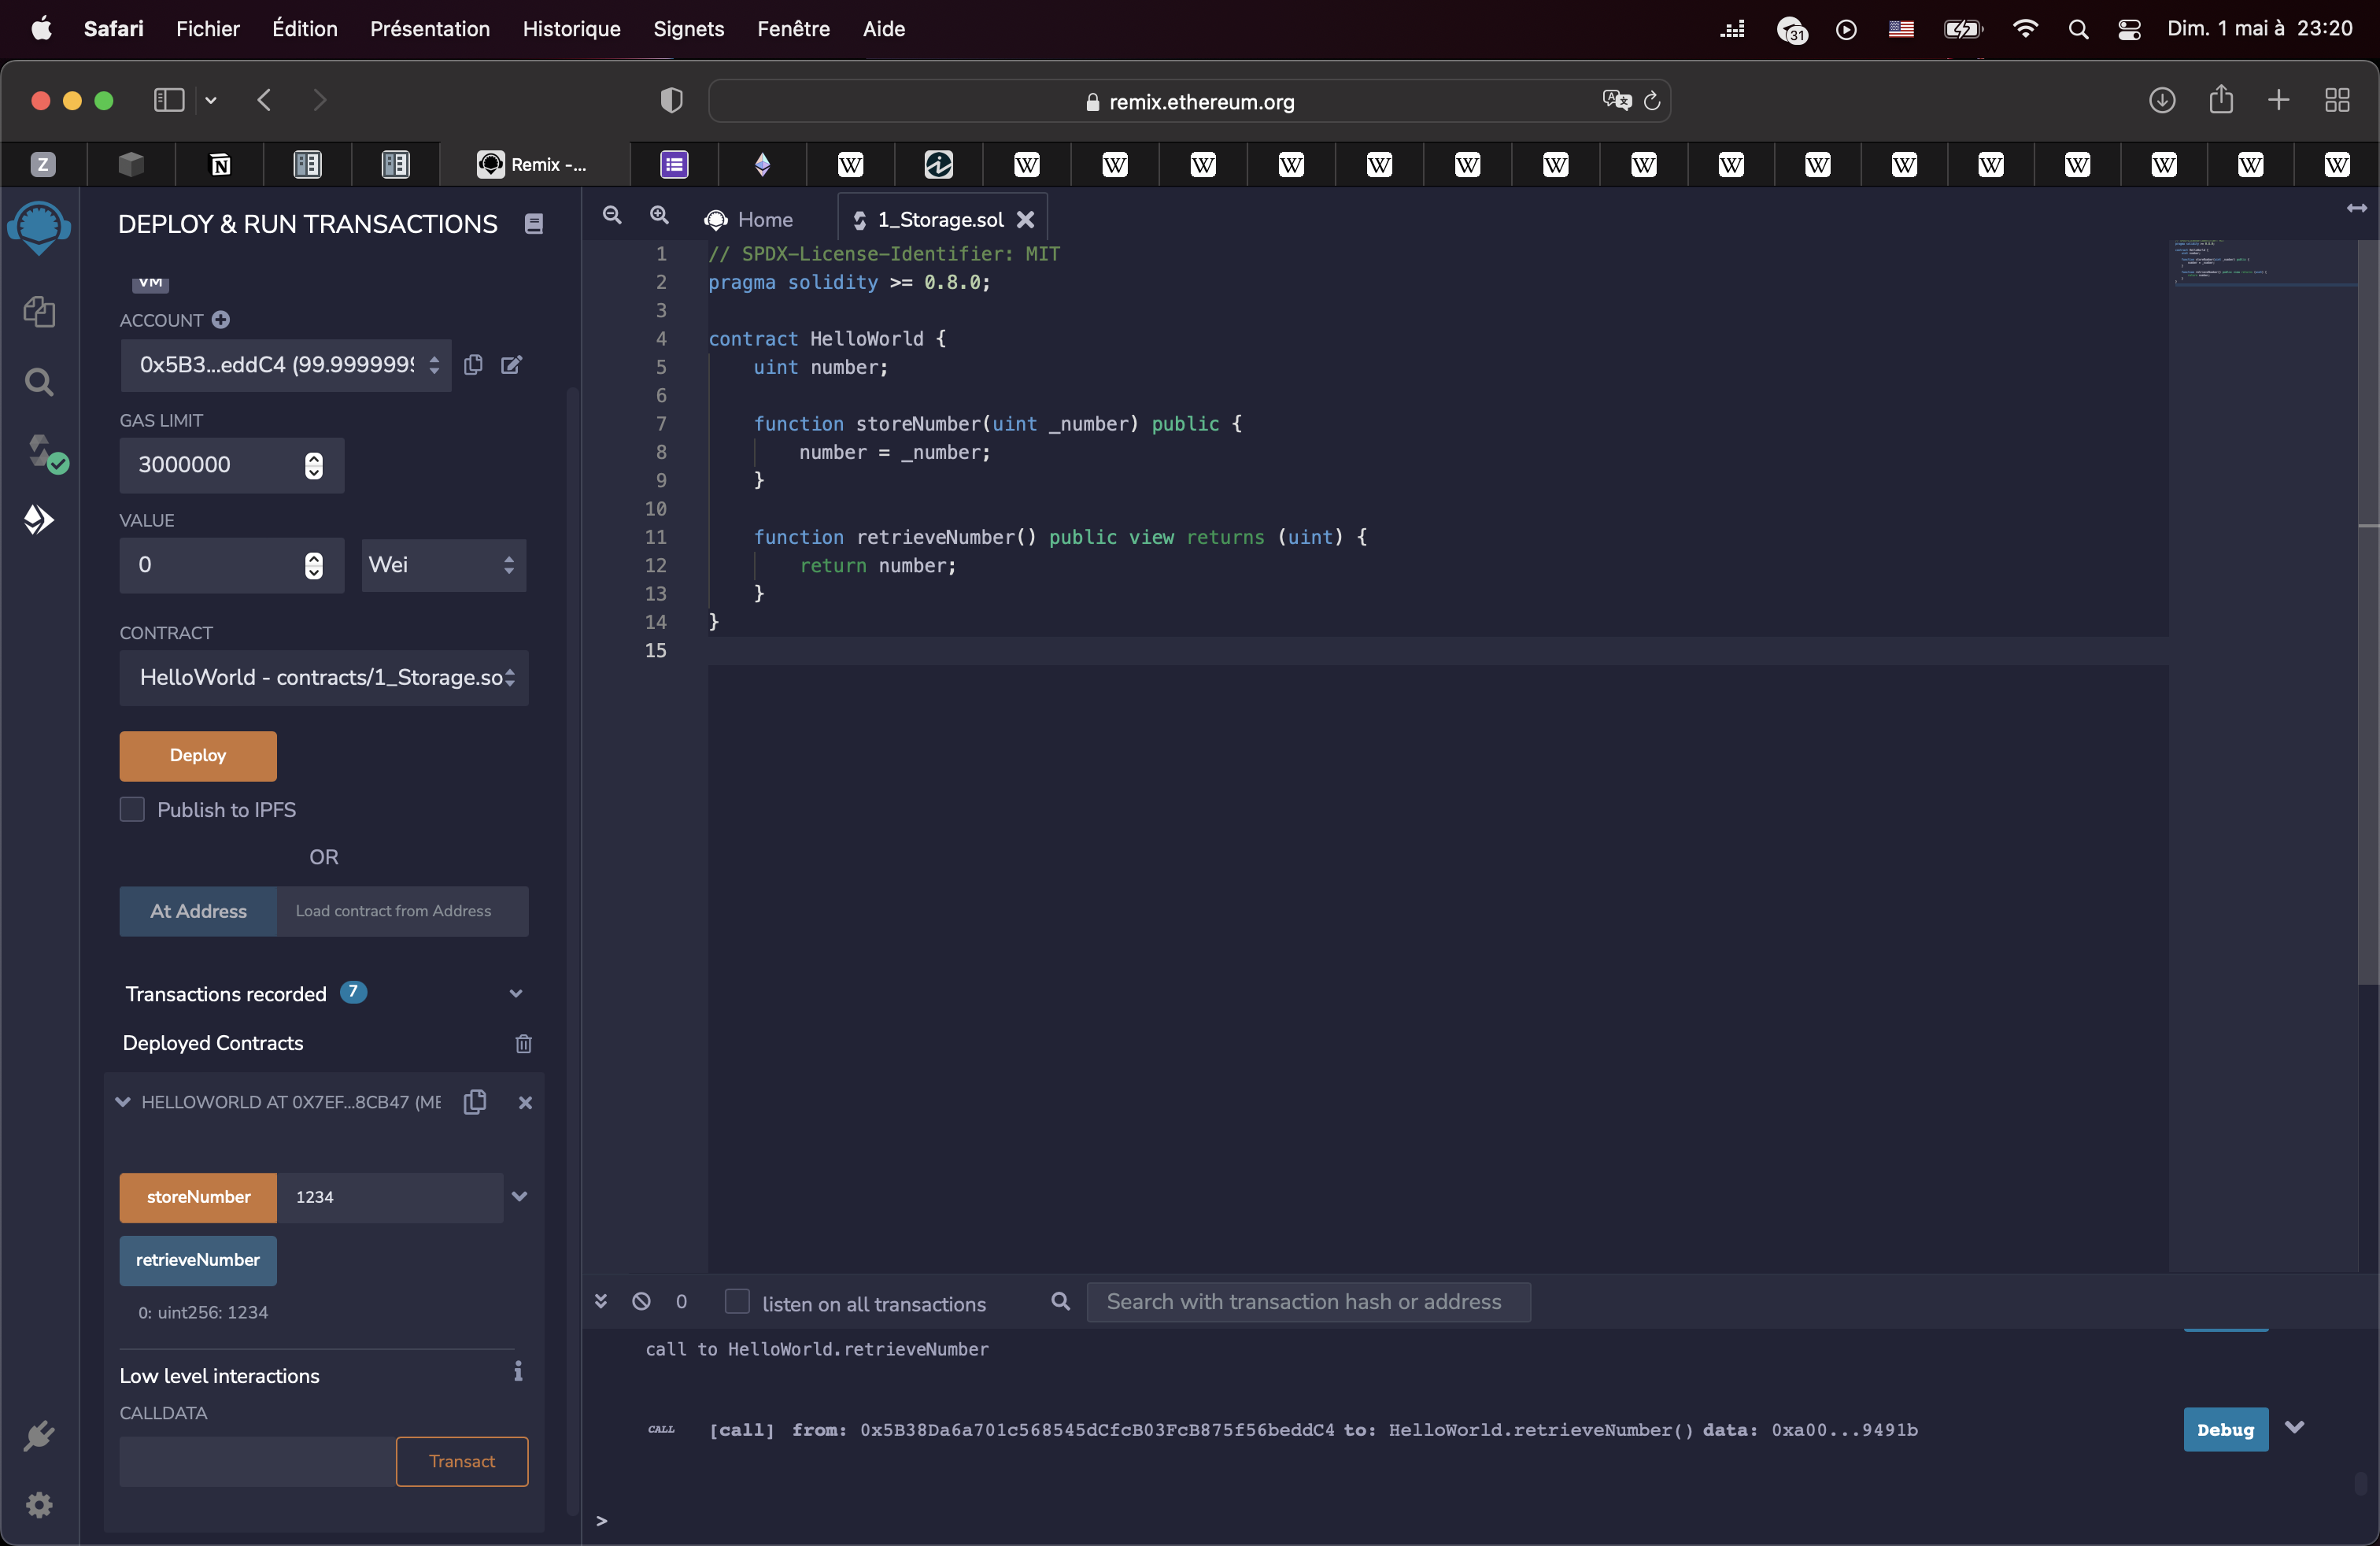
\includegraphics[width=0.7\textwidth]{screenshots/number.png}
    \caption*{The set/get contract deployed.}
\end{figure}

The second part involves modifying a Ballot contract by adding a time constraint on the vote function. This was achieved by creating the modifier \texttt{voteEnded} that checks whether the voted has already ended. Additionally, I took the liberty of declaring the variable \texttt{voteDuration} that stores the vote duration and the creating the function \texttt{startVote} that can be called by the chairperson so the vote can be started with a certain duration. The modifier \texttt{voteEnded} also checks if the vote is active, so that no votes are defined before the voting process starts. The code can be found \href{https://github.com/dbsc/zku/blob/main/background_assignment/helloworld.sol}{here}.

\begin{figure}[h]
    \centering
    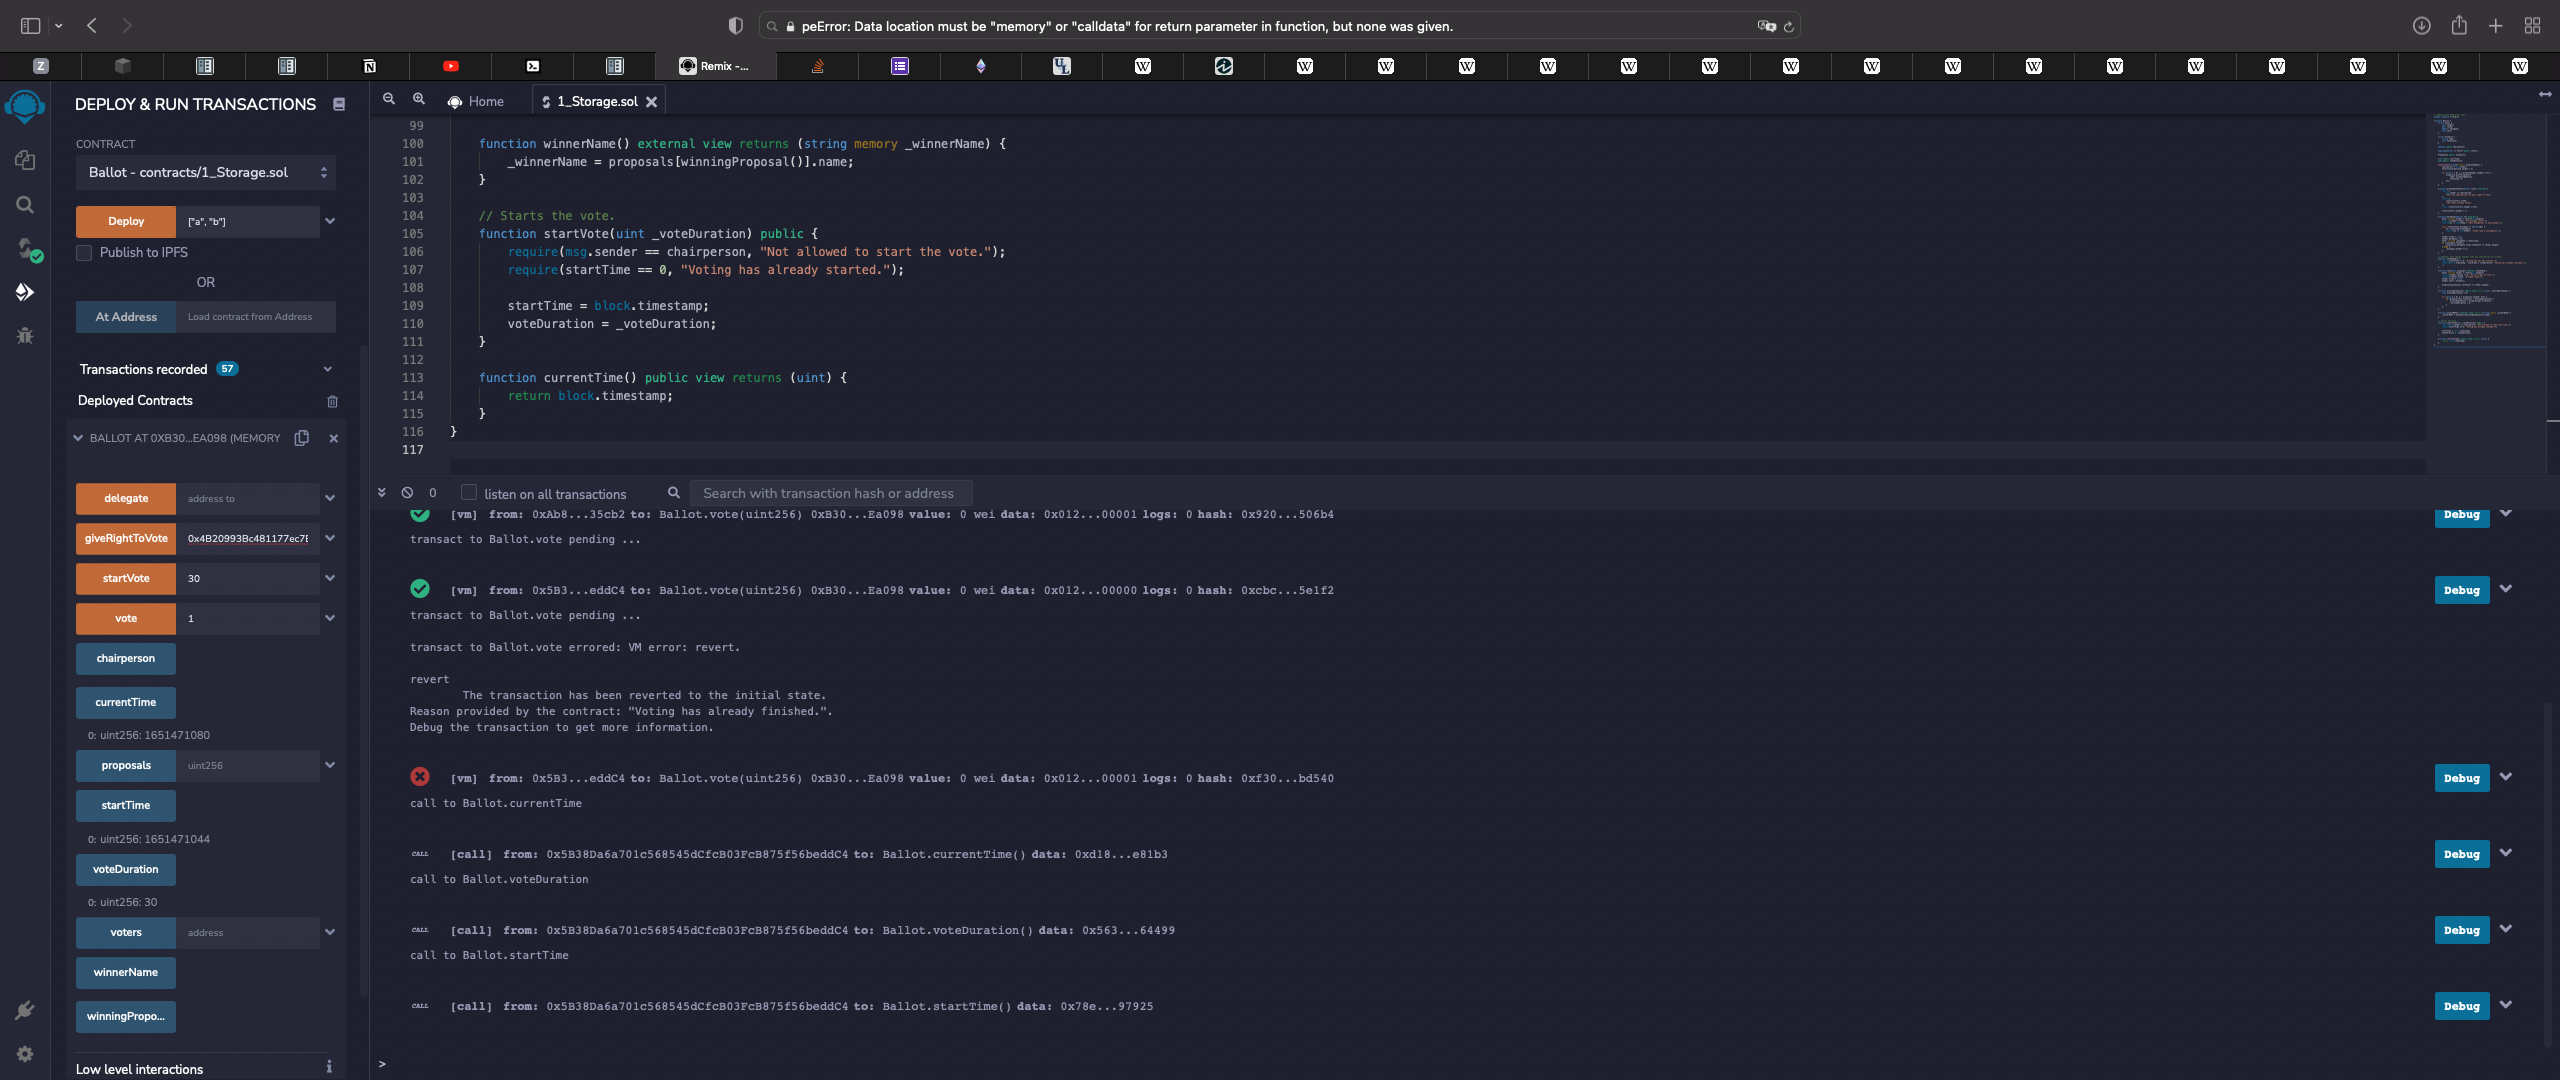
\includegraphics[width=\textwidth]{screenshots/ballot.png}
    \caption*{The Ballot contract deployed and tested for vote ending.}
\end{figure}
\end{document}
